
\documentclass[a4paper,12pt,twoside]{article}
\usepackage[a4paper,top=20mm,bottom=20mm,inner=38mm,outer=19mm]{geometry}
\usepackage{graphicx}
\usepackage{float}
\usepackage{url}
\usepackage{listings}
\usepackage{subfigure}
\usepackage{cite}
\usepackage{amssymb}
\usepackage{parskip}
\usepackage{setspace}
\bibliographystyle{apalike} 
\begin{document}
\onehalfspacing

\begin{titlepage}
\clearpage
\vspace*{\fill}
\begin{center}
\begin{minipage}{.6\textwidth}
\centerline{\textbf{\huge Gathering Atmospheric Data}}
\centerline{\textbf{\large Using an Unmanned Air Vehicle}}
\centerline{\textit{Henry Miskin}}
\centerline{\textit{\today}}
\end{minipage}
\end{center}
\vspace{5cm}
\center
\textbf{Abstract}
\center
This report looks at three dimensional energy based path planning for unmanned air vehicles in a predetermined area, with particular consideration to quality of data produced.
\vfill

\clearpage
\end{titlepage}
\tableofcontents
\clearpage

\section{Introduction}
\label{sec:introduction}

The following section outline the process in which a minimum cost route through a sample space can be obtained that provides the best data collection quality

\section{Plane Properties}
\label{sec:plane_properties}

\begin{table}[width=\textwidth]
\centering
    \begin{tabular}{cc}
    Turn Radius	& 0.1	\\
Wingspan	& 3	\\

    \end{tabular}
\caption{Table of Plane Properties}
\label{tbl:table_of_plane_properties}
\end{table}

To considere th minimum cost of circumnavigating a particular route the specifications of a plane must be considered in table \ref{tbl:table_of_plane_properties} the plane detailed in this table is the plane that is used for the entire report

\section{Energy Model}
\label{sec:energy_model}

\begin{equation}
\label{eq:energy_equation}
E=\alpha D + \beta H
\end{equation}

From these plane properties the following energy model has been definened in equation \ref{eq:energy_equation} where $\alpha$ and $\beta$ are coeficients that are determined by the plane. For the current plane shown in table \ref{tbl:table_of_plane_properties} $\alpha$ and $\beta$ take values of 10 and 6 respectively.

\section{Latin Hypercubes}
\label{sec:latin_hypercubes}

Latin hypercubes are sampling pland that provide the best space fillingness while limiting the total number of sampling points required. This is generally applied to testing of computer similations where the collection of each point is expensive. In this situation however the travel bertween the points the expensive component.

\begin{figure}[H]
	\centering
	
	\subfigure[10 Nodes]{
		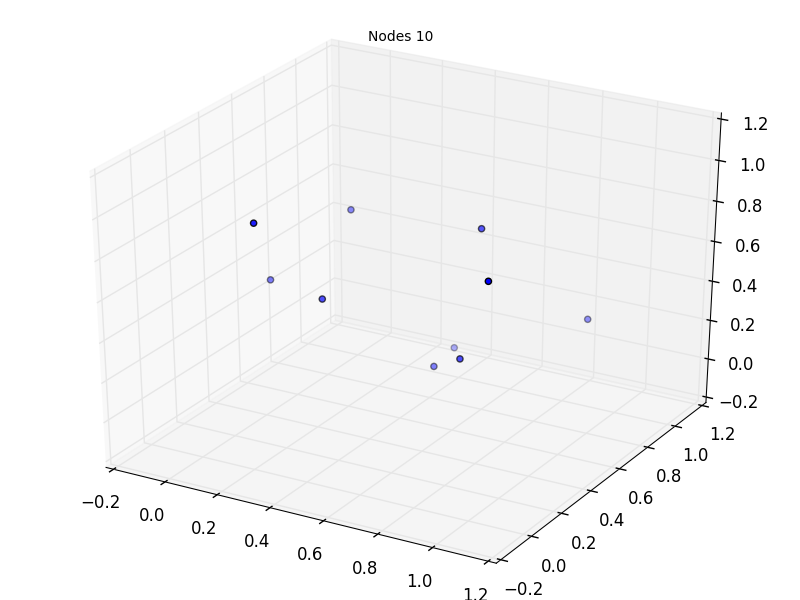
\includegraphics[width=0.4\textwidth]{figures/nodes_10.png} 
		\label{fig:10_nodes}
	}
	\subfigure[25 Nodes]{
		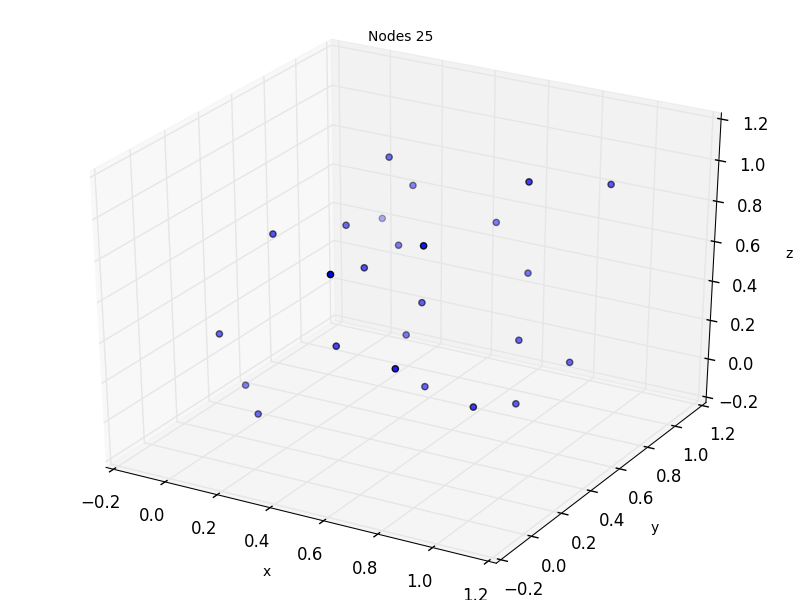
\includegraphics[width=0.4\textwidth]{figures/nodes_25.png} 
		\label{fig:25_nodes}
	}
	\subfigure[50 Nodes]{
		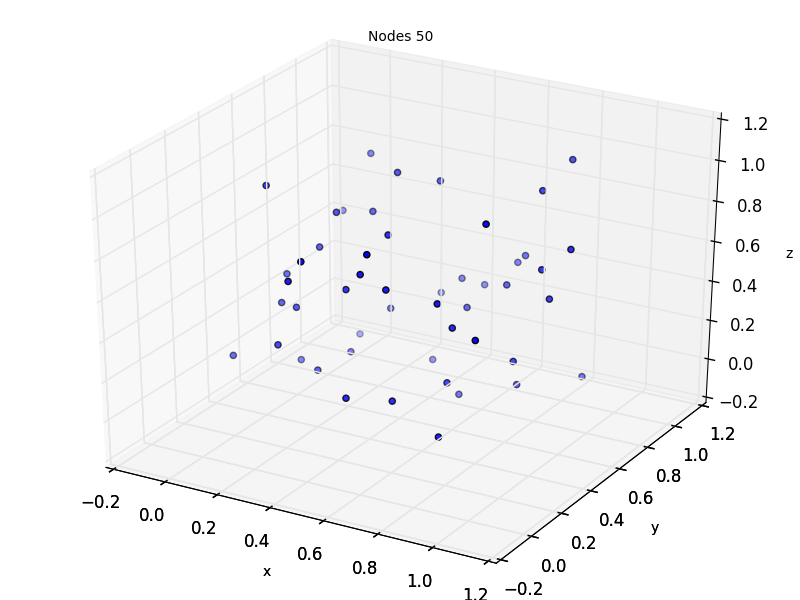
\includegraphics[width=0.4\textwidth]{figures/nodes_50.png} 
		\label{fig:50_nodes}
	}
	\subfigure[100 Nodes]{
		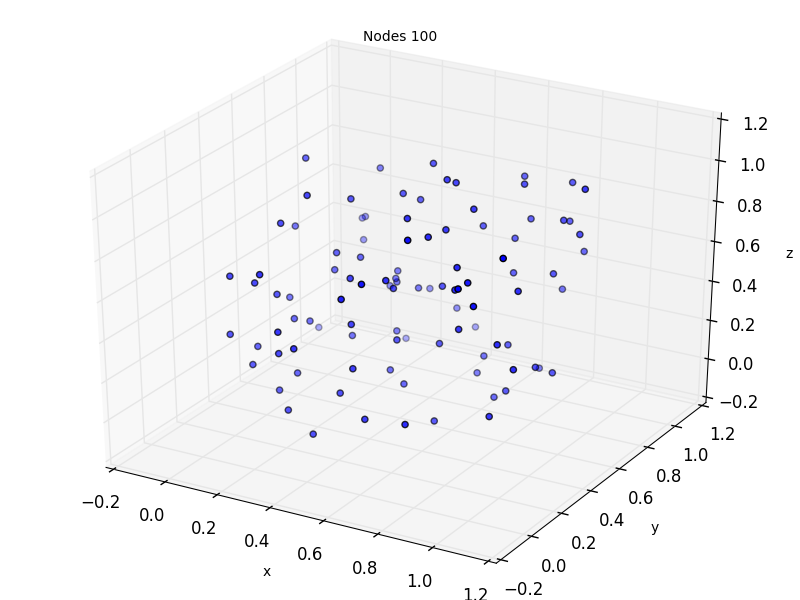
\includegraphics[width=0.4\textwidth]{figures/nodes_100.png} 
		\label{fig:100_nodes}
	}
	\caption{Latin Hypercubes with Varying Numbers of Nodes}
	\label{fig:latin_hypercubes_with_varying_numbers_of_nodes}
\end{figure}

Figure \ref{fig:latin_hypercubes_with_varying_numbers_of_nodes} shows a number of latin hypercubes with differnt numbers of nodes. All the Latin Hypercubes are within a unit cube. For collection of data in a required area these cubes can be stretched to fill the desired space. This does not provide an even spacing in each direction however means that eeach vertex of data collection is equally considered.

For this project the idea is to follow this logic to utilise Latin Hypercubes:

\begin{enumerate}
\item Specifiy area of interest to researcher
\item Estimate number of nodes able to be circumnavigated given the UAV total energy and the area of sample space
\item Fit Latin Hypercube of given nodes to sample area
\item Calcualte least energy route through the sample space
\item After first flight asses areas of encertainty to plan route through for next flight

\end{enumerate}

\section{Path Planning}
\label{sec:path_planning}

The least energy route through a number of nodes has been defined however this route assumes that the UAV is able to turn on the spot and is not constricted by turning radius. Therefore to compute the actual energy cost of circumnavigating a route the turning radius of the UAV needs to be considered. Dubins paths are the minimum distance paths given a start and end direction.

Duibins paths ar comprised of maximum rate turns and straight line segments. The following defines all the routes that are possible made op of maxiumum rate turns and straight line segments

\begin{itemize}
\item RSR - Right Turn, Straight Flight then Right Turn
\item RSL - Right Turn, Straight Flight then Left Turn
\item LSR - Left Turn, Straight Flight then Right Turn
\item LSL - Left Turn, Straight Flight then Left Turn
\item RLR - Right Turn, Left Turn then Right Turn
\item LRL - Left Turn, Right Turn then Left Turn

\end{itemize}

\end{document}
